\documentclass[UTF8]{article}
\usepackage{amsmath}
\usepackage{amssymb}
\usepackage{graphicx}
\usepackage[]{caption2} 
\renewcommand{\figurename}{图}
\renewcommand{\captionlabeldelim}{.}
\usepackage{ctex}
\usepackage{geometry}
\geometry{left=2.7cm,right=2.7cm,top=2.5cm,bottom=2.5cm}
\author{Arrow Luo}
\title{矩阵分析基础知识}
\begin{document}
\maketitle

\section{矩阵基础}

\begin{flushleft}
    设$A\in\mathbb{R}^{n \times n}$. 若存在一个非奇异矩阵$X\in\mathbb{C}^{n \times n}$, 使得
    $$X^{-1}AX=\Lambda$$
    其中$\Lambda \in \mathbb{C}^{n \times n}$是对角矩阵. 则称A是可对角化的,矩阵$\Lambda$ 的对角线元素即为A的特征值,上述分解称为矩阵A 的特征值分解或谱分解.

    \subparagraph{定理}
    矩阵$P\in\mathbb{R}^{n \times n}$是投影矩阵的充要条件是$P^2=P$,即$P$是\textcolor[rgb]{0.20,0.16,0.98}{幂等矩阵(Idempotence)}

    \subparagraph{定理}
    设$P\in\mathbb{R}^{n \times n}$是$S_{1}$上与$S_2$正交矩阵,则
    $$P=V(W^TV)^{-1}W^T$$
    其中$V=[v_1,v_2,...,v_m]$,$W=[w_1,w_2,...,w_m]$.

    \subparagraph{定理}
    投影矩阵$P\in\mathbb{R}^{n \times n}$是正交矩阵的充要条件$P^T=P$

\end{flushleft}

\begin{flushleft}
在计算矩阵的特征值时,一个基本的思想是通过相似变换,将其转化成一个形式尽可能简单的矩阵,使得其特征值更容易计算。其中有两个特殊矩阵非常有用:\textcolor[rgb]{0.00,0.07,1.00}{Jordan标准型}和\textcolor[rgb]{0.00,0.07,1.00}{Schur标准型}

\subparagraph{定理}
设$A\in\mathbb{R}^{n \times n}$,则存在非奇异矩阵$X\in\mathbb{C}^{n \times n}$,使得
$$
X^{-1}AX=
\begin{bmatrix}
J_1 &     &    &    \\
    & J_2 &    &    \\
    &     & \ddots &    \\
    &     &    & J_p
\end{bmatrix}
\triangleq J,
$$
其中$J_i$的位数等于$\lambda_i$的代数重数,且具有下面结构
$$
J_i=
\begin{bmatrix}
J_{i1}   &         &        &     \\
         & J_{i2}  &        &     \\
         &         & \ddots &     \\
         &         &        & J_{iv_i}
\end{bmatrix},
\qquad
J_{ik}=
\begin{bmatrix}
\lambda_i  & 1    &     &      \\
           & \ddots & \ddots & \\
           &      & \lambda_i & 1 \\
           &      &      & \lambda_i
\end{bmatrix},
$$
这里的$v_i$为$lambda_i$的几何重数,$J_{ik}$称为\textcolor[rgb]{0.00,0.07,1.00}{Jordan块},每个Jordan块对应于一个特征向量。

\subparagraph{定理}
设$A\in\mathbb{C}^{n \times n}$,则存在一个酉矩阵$U\in\mathbb{C}^{n \times n}$使得
$$
U^*AU=
\begin{bmatrix}
\lambda_i   & \mathit{r}_{12} & \cdots  & \mathit{r}_{1n}  \\
0           & \lambda_2       & \cdots  & \mathit{r}_{2n}  \\
\vdots      & \vdots          & \ddots  & \vdots           \\
0           & \cdots          & 0       & \mathit{r}_n
\end{bmatrix}
\triangleq R \qquad 或 \qquad
A=URU^*,
$$
其中$\lambda_1,\lambda_2,\cdots,\lambda_n$是$A$的特征值(可以按任意顺序排列)。
\end{flushleft}

\begin{flushleft}
正交矩阵的定义是$A$满足$AA^T=E$

所以正交矩阵$A$一定是可逆的,并且$A^{-1}=A^{T}$

但可逆阵不一定正交,即$A^{-1}$不一定等于A的转置。

\subparagraph{上Hessenberg矩阵:}
$$
\begin{bmatrix}
*&*&*& \cdots & * \\
*&*&*& \cdots & * \\
 &*&*& \cdots & * \\
 & & \ddots &\ddots & \vdots \\
 &*&*& * & * \\
\end{bmatrix}
$$
\subparagraph{下Hessenberg矩阵:}
$$
\begin{bmatrix}
*&*& & & \\
*&*& \ddots &  \\
*&*& \ddots & * & \\
*&*& \cdots & * &*
\end{bmatrix}
$$

\subparagraph{Toeplitz矩阵:}
$$
T=
\begin{bmatrix}
t_0 & t_{-1} & \cdots & t_{-n+1} \\
t_1 & \ddots & \ddots & \vdots   \\
\vdots & \ddots & \ddots & t_{-1} \\
t_{n-1} & \cdots & t_1 & t_0
\end{bmatrix}
$$

\subparagraph{循环矩阵circulant matrix:}
$$
C=
\begin{bmatrix}
c_0 & c_{n-1} & c_{n-2} & \cdots & c_1 \\
c_1 & c_0 & c_{n-1} & \cdots & c_2 \\
c_2 & c_1 & c_0 & \cdots & c_3 \\
\vdots & \vdots & \vdots & \ddots & \vdots \\
c_{n-1} & c_{n-2} & c_{n-3} & \cdots & c_0
\end{bmatrix}
$$

\subparagraph{Hankel矩阵:}

$$
\newcommand{\udots}{\mathinner{\mskip1mu\raise1pt\vbox{\kern7pt\hbox{.}}
\mskip2mu\raise4pt\hbox{.}\mskip2mu\raise7pt\hbox{.}\mskip1mu}}
H=
\begin{bmatrix}
h_0 & h_1 & \cdots & h_{n-2} & h_{n-1} \\
h_1 & \udots & \udots & \udots & h_n \\
\vdots & \udots & \udots & \udots & \vdots \\
h_{n-2} & \udots & \udots & \udots & h_{2n-2} \\
h_{n-1} & h_n & \cdots & h_{2n-2} & h_{2n-1}
\end{bmatrix}
$$
\end{flushleft}

\section{直接分解}
\begin{flushleft}
一般说来:求解线性方程组的数值方法可以分为两类:直接法与迭代法。直接法比较未定,但计算量比较大;所以,目前直接法主要用于小规模或中等规模线性方程组的数值求解。
\paragraph{LU分解}
将$A$分解为两个矩阵的乘积:
$$A=LU,$$
其中$L$是单位下三角矩阵,$U$为非奇异上的三角矩阵。这个分解就称为\textcolor[rgb]{0.00,0.07,1.00}{LU分解}

\textcolor[rgb]{0.50,0.50,0.50}{
并不是每个非奇异矩阵都存在LU分解。}

可以用初等变换来构造$A$的LU分解。
$$
L_{n-1}^{-1}\cdots L_{2}^{-1}L_{1}^{-1}A=
\begin{bmatrix}
a_{11} & a_{12} & a_{13} & \cdots & a_{1n} \\
0 & a_{22}^{(1)} & a_{23}^{(1)} & \cdots & a_{2n}^{(1)} \\
0 & 0 & a_{33}^{(2)} & \cdots & a_{3n}^{(2)} \\
\vdots & \vdots & \vdots & \ddots & \vdots \\
0 & 0 & 0 & \cdots & a_{nn}^{(n-1)}
\end{bmatrix}
$$
\bigskip
也可以用待定系数法来计算LU分解

在LU分解中,我们称$a_{kk}^{(k-1)}$为主元。如果$a_{kk}^{(k-1)}=0$,则算法就无法进行下去。即使$a_{kk}^{(k-1)}$不为零,但如果$|a_{kk}^{(k-1)}|$的值很小,由于舍入的原因,也可能会给计算结果带来很大的误差。此时可以通过\textcolor[rgb]{0.00,0.07,1.00}{选主元}来解决这个问题。

\paragraph{Cholesky分解}
设$A\in\mathbb{R}^{n \times n}$对称正定,则存在唯一的对角线元素为正的下三角矩阵$L$,使得
$$A=LL^T.$$
该分解称为Cholesky分解。
$$
\begin{bmatrix}
a_{11} & a_{12} & \cdots & a_{1n} \\
a_{21} & a_{22} & \cdots & a_{2n} \\
\vdots &        & \ddots & \vdots \\
a_{n1} & a_{n2} & \cdots & a_{nn}
\end{bmatrix}
=
\begin{bmatrix}
l_{11} & & &  \\
l_{21} & l_{22} & & \\
\vdots & \vdots & \ddots & \\
l_{n1} & l_{n2} & \cdots & l_{nn}
\end{bmatrix}
\begin{bmatrix}
l_{11} & l_{21} & \cdots & l_{n1} \\
 & l_{22} & \cdots & l_{n2} \\
 &  & \ddots & \vdots \\
 &  &  & l_{nn}
\end{bmatrix}
$$

为避免开方运算,可以将$A$分解为$A=LDL^T$,即改进的\textcolor[rgb]{0.00,0.07,1.00}{Cholesky分解算法}
$$
\begin{bmatrix}
a_{11} & a_{12} & \cdots & a_{1n} \\
a_{21} & a_{22} & \cdots & a_{2n} \\
\vdots &        & \ddots & \vdots \\
a_{n1} & a_{n2} & \cdots & a_{nn}
\end{bmatrix}
=
\begin{bmatrix}
1 & & &  \\
l_{21} & 1 & & \\
\vdots & \vdots & \ddots & \\
l_{n1} & l_{n2} & \cdots & 1
\end{bmatrix}
\begin{bmatrix}
d_1 &  &  &   \\
 & d_2 &  &   \\
 &  & \ddots &   \\
 &  &  & d_n
\end{bmatrix}
\begin{bmatrix}
1 & l_{21} & \cdots & l_{n1} \\
 & 1 & \cdots & l_{n2} \\
 &  & \ddots & \vdots \\
 &  &  & 1
\end{bmatrix}
$$

Toeplitz矩阵是反向对称(persymmetric)矩阵,反向对称矩阵的逆也是反向对称矩阵。
\end{flushleft}

\section{线性最小二乘}
\begin{flushleft}
线性最小二乘问题
$$\min_{x\in\mathbb{R}^n}\parallel{Ax-b}\parallel _2^2$$
其中$A\in\mathbb{R}^{m \times n}$,$b\in\mathbb{R}^m$.上式的解称为最小二乘解。
\begin{itemize}
\item 当$m=n$且$A$非奇异时,这就是一个线性方程组,解为$x=A^{-1}b$;
\item 当$m>n$时,约束个数大于未知量个数,此时我们称上述问题为\textcolor[rgb]{0.00,0.07,1.00}{超定的(overdetermind)};
\item 当$m<n$时,未知量个数大于约束个数,此时我们称问题为\textcolor[rgb]{0.00,0.07,1.00}{欠定的(underdetermind).}
\end{itemize}

矩阵计算的一个基本思想就是把较复杂的问题转化为等价的较简单的,易于求解的问题。而完成这个转化的基本工具就是初等变换矩阵,其中常用的有三个:\textcolor[rgb]{0.00,0.07,1.00}{Gauss变换},\textcolor[rgb]{0.00,0.07,1.00}{Householder变换},\textcolor[rgb]{0.00,0.07,1.00}{Given变换}。

\paragraph{Gauss变换}
设$l_j=[0,\cdots,0,l_{j+1,j},\cdots,l_{n,j}]^T$,$j=1,2,\cdots,n$
$$
L(l_j)\triangleq E(l_j,e_j,-1)=I+l_je_j^T=
\begin{bmatrix}
1 & & & &  \\
 & \ddots & & & & \\
 &  & 1 & & & \\
 &  & l_{j+1,j} & 1 & & \\
 &  & \vdots & & \ddots &  \\
 &  & l_{n,j} &  &  & 1
\end{bmatrix}
$$
向量$l_j$称为\textcolor[rgb]{0.00,0.07,1.00}{Gauss向量}.Guass变换主要用于矩阵的LU分解。

\paragraph{Household变换}
称矩阵
$$
H=I-\frac{2}{v^*v}vv^* =I-\frac{2}{\parallel v \parallel_2^2}vv^*, \qquad 0 \neq v \in\mathbb{C}^n
$$
为\textcolor[rgb]{0.00,0.07,1.00}{Householder矩阵},向量$v$称为\textcolor[rgb]{0.00,0.07,1.00}{Householder向量}

\paragraph{Givens变换}
称矩阵
$$
G(i,j,\theta)=
\begin{bmatrix}
1 & & & & & \\
 & \ddots & & & & & \\
 &  & c & & s & & \\
 &  &   & \ddots &  &  & \\
 &  & -s &  & c &  & \\
 &  &   &  &  & & \ddots \\
 &  &   &  &  & & & 1
\end{bmatrix}
\in\mathbb{R}^{n \times n}, \qquad (i \leq j)
$$
为\textcolor[rgb]{0.00,0.07,1.00}{Givens变换}。$G(i,j,\theta)$是正交矩阵,且$det(G(i,j,\theta))=1$.

\paragraph{QR分解}
QR分解是将一个矩阵分解为一个\textcolor[rgb]{0.00,0.07,1.00}{单位列正交矩阵}和一个三角矩阵的乘积。QR分解被广泛应用于线性最小二乘问题的求解和矩阵特征值的计算。

\textbf{QR分解}具有\textcolor[rgb]{0.00,0.07,1.00}{存在性}和\textcolor[rgb]{0.00,0.07,1.00}{唯一性}。\vspace{1.2ex}

QR分解可以基于\textbf{\textcolor[rgb]{0.00,0.07,1.00}{MGS过程}}、\textbf{\textcolor[rgb]{0.00,0.07,1.00}{Householder变换}}和\textbf{\textcolor[rgb]{0.00,0.07,1.00}{Givens变换}}求解。

\paragraph{SVD分解}
奇异值分解(SVD)是矩阵计算中非常有用的工具之一。
设$A\in\mathbb{C}^{m \times n}(m \geq n)$,则$A^*A\in\mathbb{C}^{n \times n}$和$AA^*\in\mathbb{C}^{m \times m}$都是Hermit半正定矩阵,且他们具有相同的特征值。

\paragraph{SVD定理}
设$A\in\mathbb{C}^{m \times n}(m \geq n)$,则存在酉矩阵$U\in\mathbb{C}^{m \times m}$和$V\in\mathbb{C}^{n \times n}$ 使得
\begin{center}
$
U^*AV=
\begin{bmatrix}
\Sigma \\
0
\end{bmatrix}
$ 或 $
A=U
\begin{bmatrix}
\Sigma \\
0
\end{bmatrix}
V^*,
$
\end{center}
其中$\Sigma = diag(\sigma_1,\sigma_2,\cdots,\sigma_n)\in \mathbb{R}^{n \times n}$,且$\sigma_1 \geq \sigma_2 \geq \cdots \geq \sigma_n \geq 0$。上述分解称为$A$的奇异值分解,而$\sigma_1,\sigma_2,\cdots,\sigma_n$则称为$A$的奇异值。

\paragraph{\textcolor[rgb]{0.00,0.07,1.00}{线性最小二乘求解方法}}
\subparagraph{正规方程法}
设$A\in\mathbb{R}^{n \times n}(m \geq n)$。则$x_*\in\mathbb{R}^n$是线性最小二乘问题的解当且仅当残量$r=b-Ax_*$与$Ran(A)$(值域)正交,即$x_*$是下面的\textcolor[rgb]{0.00,0.07,1.00}{正规方程}的解
\begin{center}
$A^T(b-Ax)=0$或$A^TAx=A^Tb.$
\end{center}
\subparagraph{QR分解方法}
由于$Q$的列向量组成$Ran(A)$的一组标准正交基,因为$QQ^T$是$Ran(A)$的正交投影算子,根据最小二乘解的几何含义有
$$Ax_*=QQ^Tb,$$
即$QRx_*=QQ^Tb$,由此可知$x_*=R^{-1}Q^{T}b$。
\begin{figure}[!hbt]
  \centering
  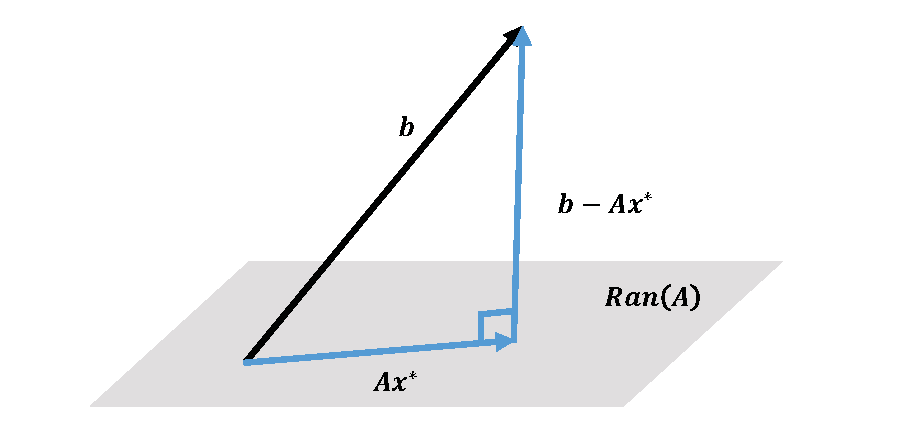
\includegraphics[width=13cm]{images/LSM.eps}\\
  \caption{最小二乘解的几何含义}\label{图:LSM}
\end{figure}

\end{flushleft}
\end{document}
